\section{\normalsize Фазовые переходы первого рода. Уравнение Клапейрона--Клаузиуса. Фазовое равновесие «жидкость--пар». Критическая точка.}
\paragraph{Фазовые переходы первого рода.} \textbf{Фаза} --- макроскопическая физическая однородная часть вещества, отделенная от остальных частей системы границами раздела, так что она может быть извлечена из системы механическим путем.\\
\textbf{Фазовый переход} --- переход вещества из одной фазы в другую при изменении внешних условий (температуры, давления, полей) при подводе или отводе тепла и т.д. \\
Величины, пропорциональные объему подсистемы называются \textbf{экстенсивными} ($V,U,S$), а не зависящие от объема выделенной подсистемыы --- \textbf{интенсивными} ($T,P,\rho$).\\
Фазовые превращения, при которых первые производные удельного термодинамического потенциала $\varphi(T,P)$ меняются скочкообразно называются \textbf{фазовыми переходами первого рода}\\
$v=\chpr{\varphi}{P}{T},\,s=-\chpr{\varphi}{T}{P}\Rightarrow$ скачкообразно меняется плотность ($\rho\simeq\frac{1}{v})$. Отлична от нуля теплота фазового перехода $q_{12}=T(s_2-s_1)$. \\
Плавление, испарение, возгонка, кристаллизация сопровождаются выделением или поглощением тепла, поэтому относятся к Ф.П. \RomanNumeralCaps{1} рода.
\paragraph{Уравнение Клапейрона--Клаузиуса.} Условия равновесия системы: 
\begin{enumerate}[1)]
	\item $P=const$ --- условие механического равновесия;
	\item $T=const$ --- условие теплового равновесия;
	\item $\varphi=const$ --- условие фазового перехода.
\end{enumerate}
Обоснование 3) : \\
	Рассмотрим двух фазную сиситему в жесткой адиабатической оболочке. Проведем в системе некий бесконечно малый процесс, в холе которого $T=const,\,P=const$ в обоих подсистемах и равны между собой, тогда:\\ $dU_1=TdS_1-PdV_1+\varphi_1dN_1;\;$\\$dU_2=TdS_2-PdV_2+\varphi_2dN_2$;\\
	Полная энтропия системы $S=S_1+S_2$, а в следствие изолированности $dU_1=-dU_2\Rightarrow\\\Rightarrow TdS=(\varphi_1-\varphi_2)dN_2$.В состоянии термодинамического равновесия энтропия максимальная, значит $dS=0\Rightarrow\varphi_1=\varphi_2$\\
    $d\varphi_1=-s_1dT+v_1dP,\quad d\varphi_2=-s_2dT+v_2dP,\quad\varphi_1=\varphi_2\Rightarrow d\varphi_1=d\varphi_2\Rightarrow$\\
    $\Rightarrow(s_2-s_1)dT=(v_2-v_1)dP\Leftrightarrow\dfrac{dP}{dT}=\dfrac{s_2-s_1}{v_2-v_1},\quad q_{12}=T(s_2-s_1)$ --- теплота фаз перехода в расчете на 1 частицу $\then \dfrac{dP}{dT}=\dfrac{q_{12}}{T(ы_2-v_1)}$ --- \textbf{Уравнение Клапейрона--Клаузиуса}.
\paragraph{Фазовое равновесие «жидкость--пар».}$\;$\\
\begin{minipage}{75mm}
	\begin{figure}[H]
		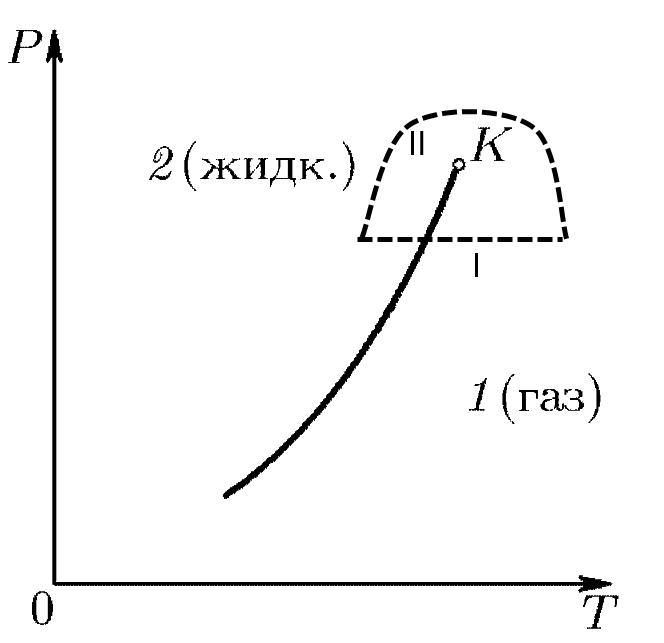
\includegraphics[width=65mm]{Klap.png}
	\end{figure}
\end{minipage}
\begin{minipage}{100mm}
	 Примем $q_{12}=q=const\Rightarrow\dfrac{dP}{dT}=\dfrac{q}{T(v_1-v_2)}$\\
	 Так как $v_1\gg v_2$:\\
	 $\simeq\left.\dfrac{q}{Tv_1}\right|_{Pv_1=kT}=\dfrac{q}{kT^2}P\Leftrightarrow\int_{P_0}^{P}=\dfrac{dP}{P}=\dfrac{q}{k}\int_{T_0}^{T}\dfrac{dT}{T^2}\Rightarrow\\
	 \Rightarrow P=P_0exp\left(\dfrac{q}{kT_0}-\dfrac{q}{kT}\right), P(T_0)=P_0$\\
	 \textbf{Критическая точка(К)} --- точка, в которой обрывается кривая фазового равновесия и исчезает разница между фазами. При наличии К всегда есть путь, в каждый момент которого вещество однородно, т.е. не возникает граница раздела.
\end{minipage}
 I --- пересекая кривую фазового равновесия (с образованием двухфазовой системы)\\
II --- в обход К (сохраняя пространственную однородность)\\
Для воды: $T_\text{кр.}=647.3\text{ К, }P_\text{кр.}=22.12\text{ МПа}$